\documentclass[twoside,11pt,titlepage]{article}
\usepackage[paperwidth=5in,paperheight=7in]{geometry}
\usepackage{fancyhdr}
\usepackage{graphicx}
\usepackage[absolute]{textpos}
\pagestyle{fancy}
\setlength{\parindent}{0in}
\setlength{\parskip}{1ex}
\setcounter{secnumdepth}{0}
\fancyhead[OE]{\small \leftmark}
\fancyhead[C]{}
\fancyhead[ER]{}
\fancyhead[OL]{}
\begin{document}
\thispagestyle{empty}
\begin{textblock*}{125mm}(0mm,0mm)
  \noindent
  
\includegraphics[width=\textwidth]{front.jpg}
\end{textblock*}
\null\newpage
\thispagestyle{plain}
\bigskip
\bigskip
\bigskip
\bigskip
\begin{center}
  \huge{\textbf{A `Psycho' Path}}\\
  \bigskip
  \LARGE{The selected short stories and articles by}\\
  \bigskip
  \LARGE{Haris Ibrahim K. V.}\\
  \smallskip
  \small{https://github.com/harisibrahimkv/psycho-book}\\
  \bigskip
  \bigskip
  \bigskip
  \bigskip
  \normalsize{Cover Design by Praseetha K. R.}\\
  \normalsize{http://imagineer.in/}\\
  \bigskip
  \bigskip
  \bigskip
  \bigskip
  \bigskip
  \bigskip
  \bigskip
  \bigskip
  \bigskip
  \small{This work is licensed under the Creative Commons Attribution-ShareAlike 3.0 Unported License. To view a copy of this license,E visit http://creativecommons.org/licenses/by-sa/3.0/.}
\end{center}

\cleardoublepage
\tableofcontents
\newpage
\begin{center}
  \section{Foreword}
\end{center}

When my friend Haris started writing this blog of his, the very name of the blog - `so-says-haris' did'nt appeal to many, including me. Most of us had a preconceived notion, about the blog, that it would be something very preachy, probably presented in a manner how an experienced man would recount his life's lessons. Little did anyone know that not only would the blog be a huge success, but it would also pave way to a book, based on the articles and stories posted in it.

Now, the blog's success is definitely due to the way the stories are written and views are presented. Since most of the stories are real-life experiences of this guy, everyone among the youth can easily relate to them. The issues raised are something each one of us faces, at some point in our lives and yet do not put in much thought about it.

In this mad race to achieve something in life, we often forget to look around and enjoy the beauty of this life, which has been endowed upon us by the supreme power. Most of us grumble and complain about what we do not possess, instead of rejoicing with whatever we do have. We usually miss out on little things in life that gives us happiness in the hope of celebrating something big.

Using this book as a medium, the author has stressed upon such small instances which are usually overlooked by us. Through his powerful way of story-telling and usage of vivid descriptions, the reader is taken through the journey of life and he realizes how beautiful life could be, all it requires is a right kind of attitude; how positivity helps human beings to embrace and feel the warmth and the eternal beauty of life. Not only this, the author makes sure that he communicates his views on the current disturbing phenomena of social networking, without being too judgmental about anything. The article `e-birth, e-life, e-grave' finds the author in an acerbic mood where he takes the readers into a hypothetical world where humans are ruled by the social networking bug. The articles `Motivation' and `Not trying, is failure', on the other hand, try to stress on how important determination, will power, perseverance and motivation are in achieving life's goal.

The stories are either author's own or his dear ones personal experiences, or are pure fiction. Some like `Salvation', `Campus life' and `Kick of fate' depict human emotions of anger, guilt, desperation and joy, whereas `Etsuko's picnic' is a simple narration of a tragic event through a little girl's viewpoint. The story `when tide flows your way' truly touches the reader's heart and `Quito San' is a rib-tickling rendition describing how organisms, other than humans, collate and carry out their so called `mission'. Overall, this book, is an out and out a `must read'.

The author's satire on various aspects of life, not only is a treat to whoever reads the book, but it also helps in connecting with him. This creation of his, is basically, his way of viewing and observing the world around him. The simple yet powerful narration holds the reader throughout, and trust me, there is'nt even a single dull moment when you are reading this book. 

So much for the book. Now talking about the author, Haris, who is a powerhouse of talent and is a dear friend of mine. A computer science engineering graduate, he is one among those who considers passion and profession with equal seriousness. Most of us tend to forget what we are most passionate about in life, and force ourselves to be a part of the rat race, but this guy makes sure he takes his penchant for writing seriously and make time to work towards developing it.

An introvert by nature, he holds his values dear and makes sure that he does justice to each and every relationship in life. An avid programmer, who prefers spending his leisure time in coding, he is also the first chairman and co-founder of ABACUS - A Bonafide Association for Computer Users and Students, an association which aims to help computer science students get acquainted to the IT industry.

His values and principles make him a true human being and a true friend, one whom you can trust with your eyes shut. So when he asked me whether I could write a foreword to his book, (since I had already read the entire book) all I could say was `yes, why not?'. It is probably the least I could do to promote a budding writer like him. Nothing more needs to be said about this guy for his excellent work speaks for him.

A delightful insight to life's experiences by an author oozing with zeal and enthusiasm, a fact very evident in his writings, this book will definitely please your inner soul and satiate your craving as a reader.\\

\medskip

\textbf{Namita Nair}
\newpage
\begin{center}
  \section{Preface}
\end{center}
Dear readers,\\

It is no secret that there are many among us who have a lot of creativity inside us. As a person living in this world, there is a lot that we see, experience and learn. As a human being, there are a lot of ideas that originate inside us from what we have learned. These ideas might be ones that have the potential to make a big difference in the world. However, almost all of us make ourselves believe that our thoughts and ideas are nothing compared to others. After making ourselves believe that, we start taking it as an excuse for not trying anything creative. ``Dude, who are you kidding? It is obviously not going to work'', you say.

This book, more than what the stories and articles within it, says ``Let us give it a shot and see what happens''.

As such, this book might not be a perfect example of literature or answers to life's philosophies. The thought that should cross your mind after reading through this is, ``If this dude can do it, why can't I?'' and this applies not only to writing, but to whatever you are passionate about. Stop taking the achievements of others as an excuse not to follow your passion. As a human, you are fundamentally different from others. You have your own thing, now just let it out. You can find thoughts on a similar line in an article titled ``Not trying, is failure'' within.

One other thing that this book stresses upon, is the fact that people are always afraid of turning against tradition. The point I'm making here is the one regarding that of having a publisher. The world has moved on and new ways have opened up in front of you.

You must know by now that Publishers tend to reject a lot of ideas and stories that come their way in the name of ``Not appealing to the public''. However, today you do not have to entirely depend on them to get your work out. What you have written is your imagination and your thoughts. The ones that you conjured up from the experiences that you had. Why should someone else stop you from presenting those to the world? All this boiling down to the point that this book is self-published and hence, it has no Publisher.

However, the blame of letting Publishers dominate artists, assuming it happens so, lies on us ourselves. The main reason being that we are not ready to promote our fellow artist's work. We tend to treat a work that has not been published by a Publisher to be a ``low-quality'' work. It might be a low quality work. But the point is that the author tried to bring out something that he had within. It is for us to support him and give him feedback regarding it. If we are to not let Publishers have the final say over an artist's work, it is us who should read, promote and support our fellow artist's work. At the time of writing this, I happen to know a handful of such people. May the world witness more like them in the future.

Another thing that this book stands for is free culture. I believe that there is no need to restrict anyone's use of this book in order for me to make money. Hence, this book is under a free license that allows you to copy, redistribute, improvise and use it for any purpose that you see fit, as long as you let others to whom you decide to give this book to, enjoy the same freedoms. Thus, the only restriction upon you is that you should not impose any restrictions on it. For people who wish to support me financially for coming out with this book, they can do so by ordering a hard copy of the book from \emph{http://pothi.com/pothi/book/haris-ibrahim-k-v-psycho-path}. Apart from the printing and binding charges, I'll get the rest of the money. The e-book is available for free download.

This book contains the articles and short stories that I wrote during the final year of my college life, as blog posts. Therefore, the articles within may relate more to Engineering students. The short stories however, has no such bias. They are from personal experiences as well as my observations around me. As a Computer Science Engineer, I support the Free Software Movement and hence this book has been developed using Latex, git and Emacs on Ubuntu 12.04. You can find the github repository at
 
\emph{https://github.com/harisibrahimkv/psycho-book}

Now, I would like to mention a few people who have been my greatest support in getting this book published. It is usually the case that there are students who are ambitious and passionate about something. However, most of the times they are not allowed to chase their dreams due to compulsion from their family. The ``If you don't have marks, you're dead'' kind of attitude. Well, my family is pretty cool when it comes to that. Mom (Safiya), Dad (Ibrahim), Brother (Noufal) and Sister (Mirfath), they have never ever posed a hindrance to whatever I wanted to do. Also, they simply did not let me go free. They would always be there to talk, laugh, advice, share and guide whenever I needed them. So the freedom that I had coupled along with my inner explorations and their guidance, is what brought me this far.

Next would be Shalin Jain, the man who taught me to follow what I love. If not for him, I wouldn't even have started writing my blog let alone, publishing a book. He is the founder and CEO of Tenmiles Corporation.

Namita and Praseetha, my proof reader and cover designer respectively. The encouragement and support that they both gave really kept my spirits up to get this done. Namita volunteered to take up the proof reading, even though she had nothing to gain from it (Hey, prepare for one heck of a treat!). When you have friends like her, you feel the world has still lots to offer you. That you can move ahead in life with the optimism that people really are good and helpful. On the other hand, Praseetha is the simple and silent girl with creativeness oozing out of her. An excellent artist who channeled her creative imaginations into web designing during her final year, she is a girl with much potential who will definitely scale up in life on a rainbow of her own colors. God bless them both.

I would like to thank all those who have encouraged and supported me with my blog. Jinu, Sharat, Manu, Poornima, Afaf, Rahul, Gouthaman, Dileep, Ajith, Anand, Ashik, Aaliya, Jijo, Aravind, Sruthi, Aparna and all of my classmates as well as my juniors who have been there for me. From the tech circle Ershad, Praveen, Zainab, Nakul, Kiran, Pramode and the others who taught me certain values in life that most importantly, included Freedom. Last but not the least, I thank everyone out there who has paid at least one visit to my blog in their life.

Here is wishing and praying for a better tomorrow.\\

\medskip

\textbf{Haris Ibrahim K. V.}

\newpage
\begin{center}
  \section{Etsuko's picnic}
\end{center}
\bigskip
\bigskip
\bigskip
``Tomorrow we're going on a picnic!'', thought the 4-year-old Etsuko, in excitement, hugging her teddy.

Etsuko was the only child of the Shimizu couple. She was a beautiful child who meant the world to them. It was almost time for starting her school education. But her Mother wanted to spend more time with her so that she could love her to her heart's content.

She would wake up in the mornings and be with her Mother while watering the garden. She had even planted a sapling which was bearing leaves. Her first experience of a new life coming into existence on God's green Earth. But little did she realize how easily one could be taken away as well.

She was aware of her parents discussing something that day. ``Grown-up matters'', she thought and continued playing with her doll house. She was aware that something she couldn't understand was going on out there. Her curiosity took her doubt to her Father. He consoled her saying that it was picnic time in their country and everyone was busy going on picnics in huge planes. That was satisfying enough for her and she was thrilled that they were going on one the very next day.

She saw her parents packing. She retired for the day and fell asleep listening to her Father reciting her a poem.

The next day she woke up early only to find that her parents were already up and walking about. She waited for a while hoping that her Mother would go to water the garden. To her disappointment, that did not happen. So she decided to water the sapling on her own and went out with the watering kettle into the garden.

She heard a few unusual cries from strange birds that day. She stroke the new leaf gently watering at its root with care. She sat and looked up at the flying planes wondering where they would be going today. The thought of new and strange places that would greet them excited her. However, she was disturbed thinking who would take care of her sapling while she was away. She arrived at the conclusion that her Mother must have already thought about it. It is a thought that all of us nurture that our parents can fix anything for us.

It was five minutes past eight. They already had breakfast and she noticed a bit of anxiety on both her parents' faces. Her Mother told her that she had asked their neighbor to take care of the sapling while they were away.

 Etsuko went out to bid farewell to her sapling.

 It was past eight thirty.

 She bent down, sat on her knees, held the newly sprouted leaf and went close to kiss it.

Suddenly she felt a rumble, something like a quake. It was natural to have slight quakes now and then and she was not alarmed. But the thundering sound that accompanied the quake made her freeze.

``Etsuko!'', she heard her Father shouting.

She looked back at her home. She saw her Father running towards her. Her Mother was behind him. She tried to stand up to run towards them. Her body rose and her limbs started to move.

But the flash came.

She saw both her Mother and Father falling down choking and screaming. She tried to shout but it was in vain. She fell, and the last thing that she saw was the leaf burning away.

\bigskip
\begin{center}
*********************
\end{center}

 In the memory of all the innocent people who died with dreams just like us, on that unfortunate day on which `little boy' was dropped on Hiroshima at 8:45am.

 August 6th. Hiroshima day.
\newpage

\begin{center}
  \section{A surprising blood test}
\end{center}
\bigskip
\bigskip
\bigskip

I was new in town and wasn't accustomed to the way of life there. I was getting along fine; making friends, talking to strangers and getting to know them and all.

However, one unfortunate day, I got the flu. My body temperature began to rise and I happened to consult a nearby doctor. He prescribed a tablet temporarily and told me to get my blood tested.

Fine. A medical laboratory was within the vicinity and I went there with the doctor's prescription.

It was a small lab. Entering into it, the reception desk was to the left, and there was a settee for the patients to wait, on the right. Someone was already sitting there and I shared the seat with him.

I expected a nurse, to come out from the room within, with a needle and a rubber tube in her hand to take my blood. However, waiting for almost ten minutes, it wasn't a nurse who came out of the room. Instead, the door opened and a tall and handsome man came into the waiting area. He was quite tall, dressed in a long black coat just like the ones that were worn by the old British royal families. A graceful scent came flowing from him and everything suddenly seemed much more joyful. It was as if there was nothing more to worry about, now that he was there, even though he was a complete stranger to me.

He had a warm smile on his face which made me feel comfortable. It was reassuring that everything was fine. With that smile on his face, he slowly came near me, laid his hand on my shoulder and sat beside me. I felt really honored that a person like him would take the time to notice me.

``You have come to have your blood tested son?'', he asked with an air of self-importance.

``Umm.. Yes, kind sir. I have come for that.'', I replied.

The smile on his face widened and I turned my face to look at the door expecting a nurse to come at any moment now.

At that moment, I became vaguely aware of a slight warmth on my neck. I realized that it was his breath. But why? I asked myself. I dared not turn and cross a man like him. I sat like a statue staring at the door itself.

His breath came nearer and nearer and then all of a sudden, ``ARGH!'', I screamed!

He bit my neck!

I jumped up in disgust and stared at him. He was sitting there calmly gargling something in his mouth. I looked at the other person sitting there and he was engrossed in the magazine that he was going through. I did not know what to do.

After rinsing for a while, he took out a test tube from his coat pocket and spat into it. There it was! Half a test tube of my blood!

``Please take a seat son. I'll give you the results in a few moments.'', he said.

I was in a trance. I sat down looking at him. He gave me a sponge and made my hand hold it where he had bitten. He went over to the reception and took a pen and paper.

He took a small sip from the test tube and after a few questioning looks and a bit of gargling, swallowed it. He wrote something down on the paper. He repeated this process until he had emptied the entire test tube.

Finally he folded the paper in which he had jotted down a lot of stuff and handed it over to me. ``Here you go son. You're fine. Just a slight fever. It'll pass soon. Go and show it to the doctor. See you.''

With that, he went back into the room. I was thunderstruck at the whole ordeal and could not decide what to do. What in the world had just happened? I had no clue. I just had to make myself believe that this was how things worked out over there. I walked out of the lab, holding the piece of paper the handsome man had given me, free of charge.

Vampires taking courses?

Seems like I still have a lot of catching up to do in this new life of mine.

\newpage
\begin{center}
  \section{Myself}
\end{center}
\bigskip
\bigskip
\bigskip

The room was relatively dark. I could make out the outline of a few figures though. I was not alone.

Light is a natural stimulus and hence when I found it shining brightly through the smallest of cracks, I knew that was where I should be heading.

At the exact moment that I had that thought, my eyes got accustomed to the darkness and the room became vaguely visible. I was surprised to see me dressed in white, standing there weak and worthless. But how could that be? I was able to see myself there in third person. I ruled out the possibility of it being a mirror because I could see that I was wrapped up in some kind of an old rag. Then who was that who shared my face? Even though he had a certain aura around him, he looked lean and completely worn out as if he was struggling to keep himself on his feet.

I was really confused as to what was happening. The last thing that I could clearly remember was seeing that old woman carrying two heavy sacks in her hands while I was on my way home after buying certain things from the market. I could not remember what happened next. But somehow there I was, watching someone like myself, who looked half dead.

Suddenly, I saw him gathering all his strength and trying to make a dash for the light from the crack. His rapid movement was cut short with a deafening blow that sent him crashing onto the floor. However, I did not feel anything but I was curious to know what was going on. I understood that the whole scenario stank of trouble. I kept my mouth shut and just stood watching.

I was wondering who landed that blow and, as if to satisfy my curiosity, I saw a hulking figure standing over the `white' me.

By then, my eyes had grown pretty well accustomed to the darkness and I could see things clearly. The new figure was not alone. There was a really beautiful girl along with him who looked disturbingly familiar. For a few seconds I could not take my eyes off her and slowly I realized that she was anything and everything that I wanted in a woman.

My thoughts were cut short by the screeching of a car's break. I did not know where it came from, but there was an awesome looking sports car in the room. The door opened and a guy got out. He looked really cool with black shades and all. Well built. He resembled the movie star whom I always dreamed of meeting someday.

He stood there mocking the helpless figure on the ground. I began to feel pity for the helpless `me' lying there. Why was this fate upon him? I had no idea. All I could do was to wait and see what would happen.

At that instant, as if with a sudden burst of energy, the figure on the ground jumped and tried taking a shot at the hulking figure. But the latter one was too strong and he again floored the `white' me. I started getting angry.

However, the hulking figure snapped his fingers and a music started playing in the background. I recognized the song instantly. It was one of my favourite songs and upon hearing it, my anger subsided.

The big guy started to turn slowly. I still could not make out his face, but I was sure he was the boss there. Everyone stood there in deep respect to him. Many people had appeared in the room by now. Most of them were on the big guy's side as if awaiting orders from him. Only one or two dressed in white were with the one on the floor and they too were as feeble as him.

The big guy went over to a table on which there was a laptop. I could make out what was on the screen. It was my favourite game. However, when he went and sat in front of it, I began to feel disturbed for I could see his face. It seemed familiar and yet strange. I went a bit more closer and what I saw froze me with disgust.

He had my face!

Yet there was so much wrong with it. Even though one could make out that it resembled my face, it had the eyes of a man who did not have an ounce of love or sympathy. The face itself was so twisted that it was horrible to behold. Only the ones who could derive pleasure out of pain and cruelty would be able to bear that face.

My mind was beginning to fill with hate, anger and disgust. I was not that ugly or cruel! My thoughts were cut short when something strange caught my eye. I saw the `white' me raising his face. I saw him looking at with me with pleading eyes and pointing to something behind me. I kept on staring at him. However, as if something pulled my gaze along with the direction at which his finger was pointing to, I slowly began to turn my head and looked behind me.

I saw the old woman just a few feet away from me, standing and panting heavily, having put down the heavy sacks. I had to help her.

With this in mind, I turned back to the room, only to see something completely amazing. The `white' me was sitting on the floor now. But he looked completely rejuvenated. All the signs of tiredness and weakness had vanished from his face and body. The aura around him shone brighter. He had a confident and pleasant smile on his face.

He was slowly raising himself from the floor when the celebrity in the black shades, standing there, saw him. ``Stay down!'', he shouted and clenched his fists ready to land a blow.

His raised arm was about to come down crashing upon the one on the floor when in the blink of an eye, the `white' me rose up landing a huge uppercut right on the jaw of the cool guy. He was taken out.

Seeing this, the hulking figure got up but the beautiful lady gestured him to wait. She went towards the `white' me and looked into his eyes. Her gaze was so strong and seductive that his eyes slowly began to lose its determination. He released his clenched fists. He relaxed and the lady slowly went near him and put her hands around his shoulders. She slowly brought her lips near to his.

``Hiya!'', he screamed and landed a fierce blow on her belly, followed by a strong right fist on her face. She was thrown away with the strength of his punch. At this, the hulking figure and his goons were on him. But the two with him had now become many. It was a small battle with many clad in white against many in black, both led by people looking like me.

However, the whites were too strong and they won the battle easily. When I looked upon the scene once again after rubbing my eyes, there was just the `white' me standing there. He looked handsome and fair. He resembled goodness and it was a pleasure looking at him. Slowly, he turned and looked at the crack where the bright light was shining from. He went towards it, put his fingers in the crack and ripped it apart, letting in a dazzling light!

I went and took the sacks in my hands. The old woman looked up and smiled at me.
\newpage
\begin{center}
  \section{Two is one!}
\end{center}
\bigskip
\bigskip
\bigskip

Thoufeeq and Hisham shared a room in their hostel. They were friends since their childhood, having studied in the same school. Somehow, as fate would have it, after clearing the competitive exams, they were thrown in together at the same college. Words could not do justice to express their joy at finding themselves at the same place, together. 

Their life was such that both of them never woke up at the same time in the mornings. Either Thoufeeq or Hisham would wake up earlier than the other. Whoever woke up first, went, brushed, finished his morning chores and came back. He then would call the other, who would do his brushing and morning chores. Once both of them had finished their `post-sleep' activities, they would happily go and have breakfast together from the hostel mess, after which they would leave for college.

It so happened that one blessed day, by all that is wonderful in this world, both of them woke up together! Well, it is life and you can't expect things to be always the same. So that is fine. But what happened next, quite isn't.

They woke up, sat up in their beds rubbing their eyes wondering where they were. After a while, both coming to their senses, got up from their beds, stretched their arms giving a yawn and went to the shelf where they used to keep their tooth brushes in a cup.

Both of them reached the shelf, extended their hands, reached the cup and you know what happened? Both went and held the same brush.

\bigskip
\begin{center}
*********************
\end{center}

Dedicated to all my friends living at my hostel. Life at my college hostel has simply been wonderful and it is something I'll proudly look back upon. It is sure to bring a grin on my face.


\newpage
\begin{center}
  \section{Kick of fate}
\end{center}
\bigskip
\bigskip
\bigskip

He is known to the world at large as Hawk-eye. His aim was to become the best at what he did and as such, when the local zone kick boxing championship came about, without even a second thought, he signed up for it.

Hawk-eye was his own master. He had no trainer nor was he interested in creating any hype. He loved what he did and would not be satisfied until he had given it his best shot.

The day of the tournament came and he was there. The fixture was fixed and the cheering began. He had to pass through 5 stages of hell to prove himself.

He had no one to cheer him. His own thoughts were his company and he got into the ring, ready to prove what he was worth!

The first three opponents he faced, were child's play for him. First, the Nameless-warrior who had to return to his momma, nameless after suffering a crushing defeat at his hands. Second, the Broken-sword, whose bone was broken due to his fierce blows! Third, the Red-dragon, who was bathed in red when Hawk-eye was through with him. And he reached the semi-finals.

Hawk-eye was lost in thought for a while. Whoever there was among the crowd who supported him, he had won them with his fighting prowess. They were not family, they were not friends. They were just amazed at his talent. True, unadulterated talent.

Thoughts were too much of a luxury at that time, for his next opponent was Super-bug! The three time champion! Super-bug was renowned for his single-hand, over-head kick. If you were to give him a fraction of free time and a small distance, that is all that Super-bug needs to launch his death blow. You don't get up once he gets you with it.

But Hawk-eye was not called so for fun. He had a hawk's eye.

Charging in went Hawk-eye! Cross jabs, uppercuts, shin blocks, front kicks, push kicks and what not! Hawk-eye went close in, never giving Super-bug his space. Blows were landed continuously on both of them. But neither of them was ready to give up. Failure was not an option for them. One, defending his honour and the other, wanting to prove his worth!

In between exchanging the blows, Hawk-eye saw an opening for his trademark. A chance to deal some serious damage with his favorite move. The lethal round house kick!

He zapped around and his leg went swirling by! But Super-bug dodged. During this move, his body came close to Super-bug's knee and wham! His knee rammed into Hawk-eye's ribs and two of them broke. Writhing in pain, Hawk-eye took a few steps back. And that was the opening Super-bug was waiting for! He put his left hand on the ground and raised his body and legs over to deliver the crushing blow. But Hawk-eye was never defeated that easily. He saw the kick coming and he side-stepped it. That round came to an end.

Hawk-eye was grievously injured. But backing down was not an option for him. That was not what he was there for.

Both of them danced the dance for 18 long minutes, each round being of 2 minute duration. And finally in the 10th round, both were exhausted. They were humans after all.

The round started. Hooks and jabs were exchanged. Still Hawk-eye stood with steadfast determination and with a hawk's concentration. However Super-bug's will was weakening.

In between the fight, Super-bug took a split second to look at his coach and unfortunately for him, Hawk-eye saw that tiniest bit of opening. His legs swirled around for the second time and BAM! It landed right on super-bug's head.

He flew from where he stood. He felt as if he was being carried and the world had stopped moving. His floating sensation was cut short with his head crashing into the ring floor...

Super-bug did not get up.

With cracked ribs, Hawk-eye was declared the semi final round winner. But there was still one more stage of hell to go through. He prayed not to black-out. He had defeated the champion.

It was time for the final round.

Hawk-eye's rival was the Fight-master! Both got into the ring. To Hawk-eye's amazement, he was suddenly aware of the situation. A hawk's instinct, you could say, for he saw that his prey was a bit lost on grasping the danger in front of him.

The bell rang.

Even before Fight-master could take a breath, Hawk-eye was upon him. A kick to Fight-master's left knee threw him off balance and round came Hawk-eye's legs with the round house! Wham! Fight-master was floored in an instant. It was only 6 seconds after the final had started. The count down was made and suffice to say, Fight-master had his fight taken out of him.

Hawk-eye won the final in 12 seconds. The record till then was a knockout in 17 seconds set by Super-bug.

Hawk-eye proved that he was the best. And he waits for a person who thinks he can defeat him. He waits, for a worthy opponent.

\bigskip
\begin{center}
*********************
\end{center}

Dedicated to my friend who lives realizing that the one thing all of us have taken for granted, Life, is a blessing.

\newpage

\begin{center}
  \section{Salvation}
\end{center}
\bigskip
\bigskip
\bigskip

He lied down to sleep. But he just couldn't. The reality of the situation sunk within him slowly, inch by inch, and he felt every second of the pain. There was nothing that he could do about it now. The time he had was over. He had wasted it. He had ignored his duty and had fallen prey to the luxuries around him and at last, only when the day came to an end did he realize he will have to pay for his irresponsibility.

He tried to close his eyes but their hulking figures punishing him mercilessly came into his mind, and it was almost as if he really felt each blow that he thought of. He tried to divert his mind to fall asleep but alas, it was in vain! Reality's grasp was too much on him. They were going to get him for sure the next day. What hope was there? Absolutely none.

He lay there listening to the pitter patter of the slight drizzle outside. He wished the world to end just then and there so that he wouldn't have to suffer the cruel humiliation the next day. Death seemed like a better alternative for him. His heart beat was rising and the agitation took away with it, all the sleep he had.

He lied listening to the music of the rain outside. But there was no enjoyment in it for him.

He suddenly heard his alarm ringing and the time was a bit into morning already. He had slept off somehow. He jumped up from his bed and for a brief second said, ``Oh please God...''.

Then he heard vaguely the maid speaking to someone over the phone. He couldn't make out what it was, so he hurried downstairs.

``Lucky kid!'', the maid said, ``They just called and said that you don't have classes today as there is a function for your senior students and teachers, on a short notice. You've got a day ahead of you.'', she ended with a wink.

His name was Shareef. He was in 6th standard.

He hadn't done his math homework.

He stood there for a while at this news, looked up with a smile and went off to get the day started.

\bigskip
\begin{center}
*********************
\end{center}

In the memory of our school days.

\newpage

\begin{center}
  \section{Quito San}
\end{center}
\bigskip
\bigskip
\bigskip

``Disgraceful, I call it!'', shouted Agronak.

``What is the world coming to these days? 200!'', and he fell silent. The court members were petrified by his rage. No one dared to raise his voice when Agronak was furious.

The draft rustling the leaves was to be heard along the room. Small and faint murmurs coming from the incube room was also audible. But no one moved. Three years had it been since they established their stronghold and things were only becoming worse for them.

After a few moments of silence, Agronak raised his voice again.

``Note it my trustworthy companions! 200 is no meagre number. Reports have come in from the Amazon that our brothers had almost felled a whole village! But here we are sitting, lost to us 200 young bloods on a scout mission at the hostel. Pah! No respect for the ecological balance do these pathetic humans have...'', He again fell into deep thought.

At the beginning, they had seen people from the hostel, drawing and leaving pools of water behind it. Very soon they understood that the humans referred to the actions that they were doing as ``vashing''. Whatever it was, the water they left behind was plenty during all seasons and a few meters away, a lot of junk food and waste were available. Agronak had found out pretty soon that all this garbage was laid behind quite a big room referred to by the humans as ``mess''. He wondered how literally it should be taken.

Anyhow, the place was apt for their spending. And they had established their stronghold behind the hostel. Three years had it been now and Agronak had risen to the top in ranks. His military tactics and training was what had kept them running over the years. But time was running low and he had thought of making Rijkar his heir. However, he was in doubt now as the last day's 200 deaths was not a meager issue. Their existence was threatened and it called for drastic measures. He feared for the worst... A deal with viruses!

Without concluding his words, Agronak went away. It was long before he came back. He went to the incube room and saw his most precious responsibility. The eggs. He walked among them. A king walking beside his loyal subjects. He knew not what their part in this was nor he knew about their fate.

He went back to the council and gave his final orders. ``Hear me out my loved ones! For a long time have we dwelled here peacefully prospering. But I'm afraid that our time here has ended.''

``We have done well on the part entrusted to us. But so many have died among us due to their poison gas and hand slaps. Oh! The humiliation! But no more. We either fall or we stand. We have to make a final stand for our lives.''

At this there rose a small murmur all along the castle walls. Especially the women were a bit louder. The sudden announcement of war had filled everyone with both excitement and anxiety. Suffice to say, most of them were in a confused state.

``Silence!'', roared Agronak. ``We are a battling race. We live for blood and we shall die for it. We fight to survive!''

At this, a loud war cry rang out from the loyal subjects. ``Long live Agronak, long live Quito San!''

Then a song broke out.\\
\medskip
\begin{center}
\emph{Day and night, do we go \\ to war, to war, to war we go. \\We strive for blood, \\till we're dead. \\To war, to war, to war we go.}
\end{center}

As soon as the song fell silent, Agronak's voice thundered. ``Let the preparations be made. On the night of the third from today shall we leave.''

A few young ones had come out of their eggs that day. Agronak, along with Rijkar, went to meet them.

``Welcome aboard my lads! How do you all feel?'', asked Agronak in a fatherly tone.

``We are fine sir Agronak. Ready for training!'', shouted all of them.

Agronak let out a contended laugh and said, ``Well, well, well, it seems you have already been briefed by Umbrug. Very good. And since you are already in such excitement, I won't keep you waiting. You shall be trained by Rijkar here. Learn fast and well children.''

``Aye sir Agronak!'', they said in a chorus.

``May your stings be pointed'', wished Agronak

Just as he was about to leave, Umbrug, the guard of the incube room came running and said, ``Oh Agronak, hail be to you. I wanted them to be ready as soon as possible. That's why I had briefed them.''

``You did well Umbrug, my dear friend'', said Agronak as he walked away.

That night, Rijkar got a chance to train his newly entrusted troop. Some fellow had come from the hostel at a rather late time for ``vashing''. Rijkar told his comrades, ``Hear me out my lads. That thing is our target'', pointing to the fellow. ``What you should beware of is his two limbs hanging from either side of his body. They have small spike like things called `fingers' at their ends. Once these spikes bend and forms a grasp and you are inside it, then God have mercy on your souls. However, from my experience, which is considerable, I have seen that most of them are not skilled at using their fingers effectively. We can simply find our way out from between them. But do not take that for granted.''

He remained silent as if in deep thought and then continued, ``But all things considered, what you should fear for your lives is their manoeuvre called `slap'. They use their limbs to slap you and in almost one shot from any of them, you'll be sent to kingdom come''. He grinned at this as he was aware of his troops fearing somewhat.

Rijkar explained to them about how to inflict maximum damage.

``Watch their necks. The veins there are your best bet. Of course, you can find it all along their body. But in most other cases, it will be covered by fat. And take care because once you penetrate their dermis with your sting, you'll have to wait for a while before you can pull out your sting and that is usually when the slap comes. So watch out!''

``Let us spread out and do some damage! Oh. And one more thing. If you wish to have some fun, you can always buzz around their ears. Its actually quite funny to see what all they do, just to get rid of the sound we make.''

The theory classes were over. Now it was time for practical classes. Rijkar went and buzzed around the guy's head first. The young ones laughed on seeing how the guy waved his hands around his head and shook it madly just to get rid of the sound. But Rijkar skilfully avoided being hit. Right when the guy had settled down a bit, there went Rijkar on to his leg and stung!

``Owwww!'', cried the human and down came his hands on his legs. Slap! But by the time the slap had come, Rijkar had returned to his troops.

``See? That's the way to do it. Now go forth my lads! Let that guy have it.''

Rijkar remained where he was and sought amusement in the performance of the newly trained lads. It was almost as if the fellow was dancing. The lads were working as a team, not allowing the guy to concentrate on one area at a time. The troop had their fun along with their training for a while on the guy and then left him alone. All of them went back to the castle along with Rijkar.

Meanwhile, Agronak was walking around deep in thought. The plan had been laid. He was anxiously waiting for his scouts to return. He went to his room to find peace. There he was greeted by Daer-jaa, the Queen, his beloved.

Both of them were silent for a while. The reality of the situation weighed heavily on them more than on anyone else. War was in front of them and that night might be their last.

``My Rose...'', said Agronak softly. There was no need for words. All that needed to be said had been conveyed in one single look. Such was the bond between them. Both owed their lives to each other. They had turned the tides of battle together. They had led generations together. They had stood side by side in battles, as a pair not to be moved by any, even though abandoned by all. Hope, they held strong till the end, and hope, had bound them together.

They sat together, hand in hand. Love was in their eyes. Slowly their old faces' wrinkles disappeared. The energy they had, in their young, strong days came flowing back through their veins. Determination swelled up in them. All the times they had been together were reflected in their eyes.

``I'll be beside you as always Gronak...'', said Daer-jaa caringly. ``I feel the end is not far and I'm not strong enough. Not strong enough to live without you anymore...''

``You won't have to, my Rose'', said Agronak. ``If we're going down, we will go down together...''

With a gentle hug, Agronak went back to the council chamber to spend a restless night.

``Sir!'', called Umbrug. ``The scouts are back''.

``Send them in'', cried Agronak.

Three of the scouts entered and gave their reports which, fortunately, Agronak found was liking to his expectation. He bade his news-bearers a good night's rest.

\bigskip
\begin{center}
*********************
\end{center}

The time had come at last. The field was bathed in the golden rays of the setting sun. The soaring eagles all had their fill and went to their sleep. The troop was amassed at the front of the castle and Agronak was in front of them.

``Here we are! To make a final stand! Here we go to avenge our loved ones' deaths...''. Agronak's voice fell. Then he continued. ``It is to war that we are going my people, maybe not to return forever. Our destinies usually lie on the road we choose to avoid it. So are you with me?'', shouted Agronak.

``Sir, yes sir!!'', came the reply in chorus.

``I say, are you with me!'', thundered Agronak's voice.

``Sir, yes sir!!''

``Good, very good. Come on then, my men. Forward march!''

The troop marched together in high spirits and at last came to the front of the gate of the hostel. The battle plans had been laid out among them that morning itself. But just when they were about to start their maneuver, a long forgotten sound was heard.

``Halt my friends! You are not without aid in this battle!'', said that voice.

Everyone turned in awe towards the direction of the voice. But to their astonishment, they couldn't find the voice's source. In this state of surprise, Agronak slowly went forward and raised his hand.

``Blessed be the day old alliances are made again! Long have we been on our own. But let us now welcome our oldest friends to join us in our battle. My friends, behold the Plasmodiums!'', said Agronak in a voice filled with both pleasure and respect.

``Hail the parasites! Hail the malaria!'', shouted the troop. When the shouting had died down, the owner of the invisible voice said again, ``Go to your destinies my lads. Rest assured that although you cannot see us, we're right beside you to do our job when you do yours. Death, to those who stand in our way!''

At this a new spirit came flowing in through the troop's veins. They were going to do this. Hope or no hope, fear or no fear, determination drove them for that was what Agronak's presence brought along with the beautiful Daer-jaa.

The troop started their maneuver as planned. The veterans were assigned the second floor as high altitude attacks required much experience and composure. The other two floors were assigned mostly in random. Except one room.

The one room which Agronak had a personal vendetta against. The room in which he had lost his beloved daughter. The room 303...

After all the troops had taken their positions, Agronak along with Daer-jaa went forward to the front of 303's window. The reason why he chose that room, was not spoken, though known. The time was at hand.

``For our glory! For the glory of mosquitoes!!'', cried Agronak. ``ATTACK!!!''

With this Agronak and his team went charging in.

``Let’s do this!''

The whole oncoming had not gone unnoticed. Most of the lights were on and many of the humans were up slapping and shouting. The war had begun. Screams and shouts were to be heard from everywhere.

Agronak and his team went forth. Just as when the battle was heating up, unsought help came. The Plasmodiums had not been idle. There came the dengue and chikun-guniya viruses. Words were not spoken among any. But now Agronak knew what needed to be done.

Swiftly he flew and punctured the first one's neck. The way was laid for their allies to do their work. And they did not fail to. The guy woke up with a shot and slap. But he was too late. The viruses had gotten in him. Agronak's team was on a roll in the room. Three of the guys in the room had been infected. Now Agronak turned his attention on the next one. His blood boiled.

But just as when he was about to inflict pain, he heard a scream. He was pushed aside and there came a zapping noise. On regaining his senses quickly, he turned around. To his horror, he saw Daer-jaa falling! He shuddered in realizing the reason. The humans had not been idle. They had invented the zapping electric bats!

Agronak flew and got her. He retreated to one of the corners with her.

``Rose!''

``Gronak...'', her voice was feeble. ``You must live for me... protect our children... I'm sorry my love. I won't be able to keep my promise... I can't be there any longer... for you...'', and she fell silent.

Rage replaced all else in Agronak's mind. He kissed his sweetheart one last time and flew back. On seeing him, the bat flew at him. He side stepped the attack. His troop was gone and only four in the room had been infected. The last and final one, the human who had stole everything from him, his wife and his daughter was yet to be infected.

Agronak roared, ``Groarrrr!!'' and buzzed around and around while the bat was being slung right at his tail. And at the final moment, the bat came straight for him. Death was in front of him. But he saw the small gap he needed. He, smiling, went directly through the gap in between the net of the bat, and went for the human's neck.

Sting! The damage was done.

Now his attention was focused on his beloved's dying wish. With the bats swishing and swirling, he dodged all of them and flew out. The war was almost over. The result needed to be waited for. There was no plan for a retreat. And hence Agronak went back to his castle.

\bigskip
\begin{center}
*********************
\end{center}


Two days later, there was news in the local papers : ``Hostels shut down due to spreading fever''.

Agronak had seen the puny humans leave, one by one. He knew his task was done. But his destiny was not yet fulfilled. He foresaw what was going to happen and ordered an immediate relocation to the canal. But he neither had the energy nor the motivation left in him.

But while the eggs were being packed up, his worst fear came true. There came the castle destroyers with their sprayers. It happened too quickly. Their castle was going to get sprayed with the toxin and that would mean the end of the eggs. He saw the only way out.

``Rijkar, arise and lead our kindred for my time has come!'', with this, he flew directly into the sprayer and blocked its nozzle. ``Go now!'', shouted Agronak.

``Here I come for you my love...'', he said to himself.

The destroyer's sprayer was blocked and he had to remove and replace his nozzle. But that time was all that Rijkar needed. He efficiently swapped up the eggs with his remaining troops and flushed themselves through the drain. Splash! Went they into the canal.

The destroyer had by this time replaced his nozzle and had sprayed away their castle. The war had come to an end.

\bigskip
\begin{center}
*********************
\end{center}


Thus ends the story of Agronak, the fearless leader. And in case you folks were wondering, I'm sitting with fever here right now and I'm the one who was the last to be infected in 303.

\newpage
\begin{center}
  \section{Campus life}
\end{center}
\bigskip
\bigskip
\bigskip


Finally, he came to his first day at college. He had waited a long time, for this day. Nervous, a bit too tensed, and above all, with many memories that he craved to relive again, he took his books in his hand, let go of a deep sigh and lugged his somewhat unwilling legs out of the room slowly. With each step he took, his heart grew only heavier. He was finally back where he had wanted to be, but was this how he had wanted? Will any of those old moments come running back to him? He had no clue.

``Well'', he thought, ``things can't be all that worse''

As in a dream, where we live for almost double the time than in the real world, his ten minute walk to the class seemed to him like a lifetime.

The trickle of water from the ruined tap in the courtyard out front, seemed to him now like an ever flowing stream that took away all the joy, sadness and the entire life of a kid with it, right from the moment he set his foot on that place. As for him, his yacht had sailed through it already and had gone into the depths. He smiled at the thought of once pushing his birthday buddy into the dirt and camouflaging him. But fortunately for the birthday boy, their Principal saw them loitering around during class time and they got busted while his friend lied still, in his camouflage.

He was nowhere near reaching his class while finishing these thoughts. Just two or three steps had he taken.

The steps seemed much more heavier for him now. Unexpectedly, he saw his two worst enemies coming right at him. But he did not feel the usual shudder through his spine. Instead, he saw himself going out to meet them.

His thoughts were cut short by a call. ``Hey newbie, having trouble finding your first class?''

It was from one of the teachers, who had helped him through his admission. They had grown to be quite close friends in a short while. ``I'll manage on my own'', he said with a smile.

Things seemed weird around him and his mind almost grew blank. Thoughts of his own seemed too much of a luxury now. He remembered the silent lad he was. And how the teachers used to tease him just for the sake of it.

He had never even once complained about it. But the wounds that he accepted were never to be healed.

How once he was made to sit in front of the class, mimicking sitting in the toilet. How that day, all of his so called ``friends'' laughed and how none of them stood up for him.

He was an entertainment tool.

How he was caught and made to strip by a bunch of drunken seniors.

All the incidents made him realize that the one thing that gave people the kick of doing things - Power. And he had it right now.

With fire in his heart and mind, his nervousness melted away and his limbs moved faster.

He almost reached his class and could see the students sitting there. It reminded him of chickens in a slaughter house.

He got into the class and all the students sat on their places. He was the boss now. He was the teacher.

``I am your new teacher'', he said, and thought in his mind, ``and boy, are you guys going to suffer'', with a grin.

\newpage
\begin{center}
  \section{When the tide flows your way}
\end{center}
\bigskip
\bigskip
\bigskip

This is a real life incident narrated to me by my dad, one fine night. I jotted it down and made it up into a story in the best possible way I could.

\bigskip
\begin{center}
*********************
\end{center}

I was sitting with my father and my brothers. We were very poor and were considered very lucky if we had anything for supper at all. One day, we were fortunate enough to get a bowl of rice soup each, for supper. By the time we were beginning to eat, we heard a knock at the door. My father opened the door and there stood, a very weak and thin man, shivering with cold. He begged for some food.

My father, without saying anything to him or to us, welcomed him in and poured a fraction of soup from each of our bowls into another bowl and offered it to him. He drank it with much gratitude. Before going away, he blessed and thanked us with all his heart.

Naturally, out of curiosity, we all asked father who he was. Our father replied:

``Children, I've been working for my livelihood since I was five years old. Once, when I was full of hunger and exhaustion, I went and begged one of the shop owners for some food. He treated me very kindly. Instead of giving me food, he whipped me five or six times and made me run for my life. And do you know what is the most interesting thing that has happened to me over the past few years? It happened just now. The man whom I gave food to just now, was that shop owner's son.''

\newpage
\begin{center}
  \section{The Prophecy of Amelyah}
\end{center}
\bigskip
\bigskip
\bigskip
The battle had raged non-stop for seven days now. The Raikans had defended their village bravely from the evil of Bola. Aazmir, Son of the River as they called him, stood firm with his sword drawn. Through day and night, hunger and strife, pain and agony, the Raikans had held them off through sheer power of will. However, they were getting exhausted. Even though Aazmir and his friends had a will as strong as iron, they were only human. Their body's each and every cell had been tapped to their marrows and the Bolan army kept on coming at them by thousands. They were outnumbered.

\bigskip
\begin{center}
*********************
\end{center}

The Raikans were a peaceful tribe along the coast of the river Amelyah. Although they had lived through wars and battles from the olden days, they had finally settled down to live a life of peace. Through years, they had grown to occupy acres of coastal land. They thrived there, and did not interfere much in the matters of the outside world, because they did not depend on anyone for their sustenance. However, on the day of the full moon every month, one among them would set out on a journey to bring back whatever news they could gather.

Their tribe was wrapped in God's green beauty. If a soul ever wished to find peace at heart, then this was the place that would bind his soul to the essence of the murmuring green that slowly swayed with the gentle breeze.

The ever flowing bed of pearls that served as the resting place for the heavenly stars at night was the river Amelyah. Flowing from the heavens, she would bring happiness to the Raikans. They would feel the energy and soul of the Nature with her enchanting sound. She would flow along the rocks, soothing and shaping them as if with the hands of a skilled craftsman. It is said that the sorrows of the people are washed away by her crystal beauty. She was sacred and they would gladly give their lives for her. There was a prophecy regarding the river that a time would come when she would rise up and pass judgment on all that is evil.

Aazmir was the son of Thajir and Theheja. Even though rituals were held at the birth of a child that would bless the little one with the spirit of Amelyah, Thajir was adamant that his son should be born on the banks of the river itself. His wish was made true and Aazmir was born, to be called, the Son of the River. A blessed child he was, for his strength and will, rivalled even those of the men there.

He loved to spend time along the banks of Amelyah and would sit there for long hours looking into the clear water and enjoying its gentle sound. Sometimes immersing deep in thought, he would feel as if his soul was taken to distant lands by the waves of the flowing water. He would only come out of his dreams when some of his friends came and called him. His love for the River was much greater than any of the Raikans.

Their beliefs and rituals were confined to Amelyah. To them, she was God and whatever they had, was her gift. They never took it for granted. They preserved and nurtured Nature with such care and love. Often people who bathe in the river of love got into a trance for a few seconds. It is said that they would behold a certain vague image of a galloping beast with a rider mounted on it. It would pass through, bathing the entire village in a pool of crystals and the green would hold their heads up high in great reverence and respect. The trance would end in a few seconds. However within that time, they would have experienced a feeling so strong that their courage would become like mountains that hold the Earth down.

\bigskip
\begin{center}
*********************
\end{center}

Years passed. It was one day, during the second month of fall, that the Raikans noticed the slight tint of black among the beautiful currents of Amelyah. Their hearts were disturbed upon seeing their God's beauty being scarred. Moreover, with each passing day since then, the black currents started appearing more and more. They did not know what the reason for this unfortunate happening was and their concern grew more with each passing day.

On the next day when the moon rose up and high in his full vigor, it was time for one among them to set out on the journey to bring back whatever news he could gather. With the black currents infesting Amelyah, it was crucial for the Raikans to know what motion in the world outside triggered it. As was the custom, the Village elders, along with the young men, gathered at the clearing along the bank. The moonlight illuminated the land. They could see the reflection of the moon blotched by the dark currents flowing through Amelyah. With haste, they began the discussion.

One of the elders spoke, ``Miselyah shrib'a". In the Raikan tongue, it was their form of greeting. He continued. ``Brothers, it is time for one, among us, to journey forth into the lands outside. Even though, as usual, his mission would be to bring news from afar, this time he will be burdened with the duty of knowing what foul being is the cause of this!", he said pointing to the River.

After pausing for a few moments, he said, ``Who, among the bold and brave, shall volunteer to go forth?". Usually, many hands would go up, for the curiosity to know what was there in the world outside among the young, was so great. However, that day, no hands were raised. Some unknown power had scathed their God. As much as all the love they held for Her, the fear of facing a power so strong instilled fear in their hearts. There was silence and only Amelyah's sound could be heard.

``I shall go!", said a voice at the back, breaking the silence. Everyone turned around and they saw Aazmir, standing up, strong and bold, as mighty as the legendary Warriors who once fought for the survival of Raikans. ``For the love of Amelyah and all that we hold dear, I shall go forth and seek the cause of this blasphemy", he said with an air of confidence and courage. His elders looked at him in wonder, for it was the first time that they were seeing a young one speak so boldly.

``Aye, thou speak well, oh Son of the River", the elder said, ``For courage is what we need at times like these". He looked at all the others there and asked, ``Do I have the consent of all?". The silence prevailed. The elder, understanding the situation at hand, spoke. ``Aazmir, you shall go. The people of Raikan place their faith in you. Bring us news of what hurts our pride. With the prayers and blessings of Amelyah, you will set out with haste. The counsel has spoken. The rider has been chosen. All hail Aazmir!"

``Shrib'a iktha, siya Aazmir!", said the gathering uniformly.

The preparations for his journey were made quickly. He went forth with a heart laden with sorrow, knowing an unknown source had harmed his love. However, in order to leave the Raikan tribe, one had to cross the bridge of Garand. It was the only way on foot to the tribe. If not that, one would have had to swim across the currents of Amelyah in order to get to the village. When he reached the bridge and was about to cross it, he beheld the black currents flowing ever more strongly. He turned his gaze away from the unholy sight and sped on his way.

\bigskip
\begin{center}
*********************
\end{center}

The people of Raikan became restless as they watched the black currents of Amelyah grow stronger. None of them dared to touch the currents and as such their soul’s energy was being drained away constantly. Their only consolation was the pampering murmur of Amelyah, that still sounded with the sweetest of tones, day and night.

On the night, after a fortnight since Aazmir had left, the Raikans' patient waiting was rewarded when they heard the whistle of the traveler from afar. But they knew something was wrong. The sound of the hoofs was not peaceful. The traveler was hurrying back. Aazmir was galloping back with great speed and that made his friends uneasy, so as to what news drove him back with such haste.

They saw him coming at a rapid pace and faintly could make out him shouting something. As he approached nearer, his uttering became clearer and what they heard, made them freeze with horror. It was a word not to be spoken, a word so unholy that the tides of time had buried it deep within their history, a word they did not expect to hear even during their worst nightmares.

``Bola!"

They were not able to see Aazmir clearly due to the night's shade. When he got close to them, they beheld his garments, which were burnt and marks of black covering all of it. Still, they were not ready for what was yet to come. Aazmir removed his mask slowly...

And there was the mark of Bola on his face.

Bola was the evil of lands that was prophesied to come at the times of ill bearings of the world. The evil that would slaughter beauty and spread chaos among the kind hearted. The destroyer of life as it is, and the binder of one's soul to hell. Bola was inhuman.

The mark of Bola was made on the people whom they captured and wanted tortured for life. The mark, once put on a man, would bind his soul to the depths of hell. The chaos and flames of hell would slowly burn his soul, a little at a time. He would feel the pain of his soul, his life burning away, inch by inch without feeling even the slightest of pain to his body. There was no cure but to writhe in agony until one's soul was completely burnt away from within.

\bigskip
\begin{center}
*********************
\end{center}

The fear that the Raikans had, began to vanish. All the fear and pain were masked by their love for Her and that was what kept Aazmir on his horse till he reached back. He delivered the message. He told them that Bola had already made their mark on certain places and had captured most of river Amelyah. But in order to spread their evil, they needed the final part of the river. And that was the part protected by the Raikans. Bola was on their way for the final piece of their puzzle.

On hearing this, the Raikans' blood boiled. They were not just going to fight until they stood dying on their very feet, but they were going to make sure that the Bola would never get the river completely. With this in mind, they went back to hold discussions on what was to be done.

Amelyah was their life and death. She was the bearer of purity and love, and they were certain that if they were to stand a chance against Bola, then it would be in Amelyah's presence only. They would barricade the bridge of Garand and defend valiantly over there. If, during the worst case, the barricade was to give way, they would fall back to the village and swiftly, destroy the bridge behind them, forcing the Bola to cross the river. At that time, the Raikans decided they would kill the Bola before they crossed the river.

This was agreed upon and the Raikans chose their strategic positions wisely. Since they had the heritage of battling numerous wars, they knew of the military maneuvers. The war veterans polished their skills once more and started commanding the men. Archers, Swordsmen, Spear-men and all those who could wield a weapon were summoned. They were quick to learn the art of fighting as it was already in their bloods.

The village elders found the energy of the olden days flowing through their veins once again. They trained the young bloods day after day. Among the new generation, Aazmir, even though tormented by the mark, was the first to master the skill of swordsmanship. His strokes were swift and flawless. His courage and valor was greater than that of any. More than anything, he loved Amelyah more than his life itself. That love kept him alive.

They knew their weapons would not cause harm to the Bola. As such, their mind and soul, and its purity was their only real weapon. Along with the blessings of Amelyah, they placed their hopes in their belief and faith. They would pray each and every day. After training, they would sit and listen to Amelyah's voice. Their spirits would find peace and their souls would be rejuvenated. Aazmir would stay longer, as if he was talking with Her.

One day, after everyone had left the river bank, Aazmir remained there. He slowly walked near to the waters and stood just beside it. ``Oh Amelyah", he said, ``Bearer of love and sustainer of purity, my soul burns. Not from the mark the evil Bola placed upon me, but from the thought that your beauty have to suffer such a fate. I live for thee and I pledge my life to thee. I promise that I shall not allow those foul creatures to take you!"

As if She had heard him speak, suddenly the black currents started shifting towards the opposite bank bringing the pure and refreshing waters of the river nearer to them. It was as if a straight line of divide had been drawn in the middle of the river with one side pitch black, and the other, heavenly white. Aazmir understood the sign. He shouted, ``Raikans! The moment is at hand! Amelyah has spoken!"

The Raikans rushed towards the river and saw the omen. ``Prepare for battle!", shouted Aazmir. With haste, armors were put on, swords were drawn, arrows fixed and they manned their positions. The barricade was set up earlier itself and the men assumed their tactical positions around it. They closed their eyes for a moment, heeded the murmur of the River, prayed and opened them again.

From the very distance, they could vaguely make out the faint outline of the dark Bola army approaching...

\bigskip
\begin{center}
*********************
\end{center}

Even after the sixth day of the battle, the Raikans held them off. As long as the Bolas were trying to hurt Amelyah, the fire kept burning within their hearts. However, they were exhausted. The inhumans did not die. Only repelled and rendered powerless with the purity that the Raikans held true, which was being put to the test. The army of Bola was persistent and kept coming at the Raikans. They did not get tired and battled day and night. The continuous battle had weakened the Raikans physically and many of them had fallen, to be carried back to the village.

Aazmir stood stern and rallied the remaining Raikans. However, he understood that guarding the barricade any longer would only cause more harm to his people.

``Fall back, fall back!", shouted Aazmir. The Raikans let forth one final wave of attack, pushing the Bolan army back, and they retreated back to the village, leaving the Barricade. Aazmir followed his men and when the last man had crossed the bridge, he carried forth his orders. He cut the rope that held the bridge.

The bridge collapsed, sending the few Bola that followed them crashing along with the bridge, into the river. When the pure waters touched them, they screamed and choked. Gasping for air, they splashed their way to the other side of the River which had now the black currents flowing through it.

The Raikans stood in front of their village and the Bola on the other side of the river. Aazmir realized that continuing the fight in this manner would only lead to their demise. He lowered his sword and thrust it onto the ground. He bowed his head, resting his forehead on the hilt of the sword, and started praying. His soul hurt now, more than ever.

On the night of the seventh day of the Battle of Garand, suddenly the Bolas seemed taken aback. There was a deadly silence within the realm of battle. All the rage that the Bolas were attacking the Raikans with, seemed to be sapped away from them. The huge army of the Bolas suddenly seemed to be distracted at some strange phenomenon that was happening without the Raikans' knowing.

The Raikans also started to feel a great sense of inner peace within them. A feeling that no one had ever encountered before. A feeling of hope and love. They felt a new energy flowing from deep within.

A gentle breeze started to sway the green trees around. They too seemed to have been roused by something strange and it was as if they had grown taller and higher in a few seconds.

The feeling lasted in the battlefield for a few minutes which was broken by a horrendous and fearful war cry from the Bolan army. The Raikans readied their swords. To their horror, they saw the Bola getting down into the river. The black currents that the Bola stood upon slowly started spreading through the River, over to the banks close to the village. Through that spread black current, the Bola started crossing.

Aazmir drew his sword and ran to cut off Bola from crossing the river. His men followed him, shouting. However, before Aazmir could make it, the black currents had reached the bank near to the village. Aazmir, followed by the Raikan army jumped into the river and swung at the Bola there. There was something different and the Bola seemed desperate to get over with the battle. They came at the Raikans in huge numbers, charging with fury.

The Raikans fought bravely. After all, they were standing in the River of Love, Amelyah. However, they did not know how long they could hold out. Aazmir took down many Bola, but the mark was burning within him. He started to feel exhausted. He started to see black spots. He was slowly losing his grip on himself. In this state, a handful of Bola came and placed their hands on him.

Aazmir screamed with pain. He could feel the final remaining parts of his soul burn away with their touch. He held his sword tight and took one last, loving and caring look at Amelyah. He dropped on his knees, and fell, into the river of love.

A brilliant flash of light suddenly threw those Bolas in the river up in the air. There was a gush of strong wind and suddenly, the clouds of the sky made way for the shining moon. Amelyah started shining and sparkling as if by heavenly magic, which made the Bola go mad with fear.

The river slowly started rising. They could almost hear as if Amelyah spoke something to them. The river started swaying as if it was alive. The Raikans started to feel rejuvenated. ``The prophecy!", cried one among them. ``The river is rising. Stand your ground men! Amelyah has heard our prayers!".

The Bola army had regrouped on the opposite shore. Seeing the strange phenomenon, they panicked. With a sudden war cry and a horrifying howl, they rushed forth to finish off the Raikans in one swift wave of attack. They came charging towards the village, crossing the river. Just as they reached the place where Aazmir had fallen, a fountain of water rose up in front of them, lifting Aazmir high up. The moon light shone on him and the Raikans stared at the happening in awe.

From afar, there emerged the figure of a water beast out of the risen water. It galloped towards the fountain and in a swift jump, landed on top of it. They saw the water covering Aazmir entirely. It swirled around him and covered him completely. Suddenly the fountain dropped into the river with a huge splash. The water sprayed in all directions. And when everything had settled down, there he was..

Aazmir, the Water Rider! With Amelyah's water sword in hand and mounted on the Water beast, he slowly raised that sword.

The Raikans who had experienced the trance while bathing in the River knew what they were seeing. The vague image of the galloping beast with a rider mounted on it was there now, standing right there in front of them, for real. They shouted out of happiness, ``It's the Water Rider, the Water Rider!!".

Aazmir charged into the midst of the Bola with such fury that they shrieked and started to run. Their hearts were filled with fear for it was Aazmir's love for Amelyah that was coming at them with such power. They could not face it for they knew not what it was. Aazmir shouted,

``Come oh Raikans! Holders of purity and lovers of Amelyah! Your protector is here and your spirits and minds have been kindled with the love of Heaven! Let us drive these creatures of ill omen out once and for all!"

With this, he thrust his sword into the river. Suddenly, all the weapons wielded by the Raikans blazed with a watery flame around them. He turned around and charged into the Bolan army causing havoc. His sword massacred the Bolan army. His strokes passed through them and turned them into dust. Not anything that the Bolans did could hold the Water Rider back. He cut through the entire black army like a comet shining in the dark skies! The Raikans followed his lead and cleansed the evil of Bola. The week long battle of Garand had finally come to an end. Love had won over hate.

When the sun rose on the 8th day morning, the black currents had disappeared and the sun shone brilliantly on the River like a diamond's gleam. The River was back to normal and the Raikans were tending to the injured along its banks. The Women and Children were preparing a feast to celebrate their victory. While everyone was talking about how fate was on their side, Aazmir stood alone at the edge of the village, looking at the River...

She had cleansed the mark of Bola from him. She chose him to become the Water Rider and fulfill the prophecy. But had he deserved to be saved? His travel on the night of the full moon was not uneventful. His mind reflected upon how the Bola had captured him. His heart felt a bit heavy...

The true spirit and love that they had held for mother Nature had won, for now. Amelyah was back to what it was, for long years to come.

\newpage
\begin{center}
  \section{Shifting gears}
\end{center}
\bigskip
\bigskip
\bigskip

This article is based on the teachings of Mr. Ambujakshan Nair, or Ambu as he likes himself to be called.

\bigskip
\begin{center}
*********************
\end{center}

Shifting gears, an action we all are too familiar with. When there is a hill ahead, we down our gears and when there is a straight road ahead, we up our gears, right?

This was the essence of his entire talk. How well we are able to shift our emotional gears, and how well we behave in the company of various people. One might be a cool, care-free guy having a rocking persona; which is fine when he is around his friends. But when you are in the presence of someone with an authority, like your Father, Mother, teachers or even when you are working in a firm, you have to shift your emotional gears to adapt to it. If you try to ascend a hill in 4th gear, you are not going to make it.

Most of us say you have to be who you are, wherever you go. But that is just the irresponsible way of making an excuse just like the ``lashing'' and ``withdrawal'' of Wolverine. I remember once helping one of my friends with the answer to that. It might be the dumbest thing, but my thoughts on facing a situation were evolved from one of my favorite characters, Wolverine. In one of the stories, it is explained to him by a long dead love of his, about how he reacted to various situations in life. He had just two basic ways - Lashing out or withdrawal. This was because he was not ready to get emotionally hurt by facing the situation.

Just as this thought came into my head, Ambu sir came with his version of it.

``You can react, respond or fall back to the situations in life''.

Lashing out = React.

Fall back = Withdrawal.

And the third one, respond, was the advice that I had given my friend. To face it, process it in your brain and the result should be the outcome of that processing you did.

We are all busy believing and taking for granted what others say without even putting an ounce of thought into the matter. But Ambu sir quoted his own example to explain how emotional gears need to be shifted.

He is a busy marketing person and is involved in a lot of businesses which keep him occupied all through the day. He is a serious professional when it comes to dealing with his clients and shows a lot of authority when it comes to fulfilling his role. But, he is a father too. A father to two sweet girls as of now. One, two and a half years old and the other, eight years old.

When he goes to them, he can't be, what he was, in his business. All his humongous degrees, consisting of all the English alphabets, means nothing to those two cute girls. They want him to play, care, be foolish, tell them stories and so on. So he shifts his emotional gears and adapts to his children and family leaving all the professionalism behind.

As such, being who you are, wherever you go doesn't mean the way you posture yourself to others I guess. It means the beliefs and morals that you carry within you. Your belief in religion and God. The virtues that you have learned from your masters. I mean, I still haven't figured out the exact meaning of ``Be who you are wherever you go''. It has a fine line that divides the things to which it applies and to the things which it doesn't.

There are some among us, 20 to 22 years old, who talk like they have experienced everything and they have figured out all the answers to life's questions. Some people saying you have to be happy all the time, others saying you have to be cool all the time. They say you shouldn't introspect, you shouldn't sit and think of the things that make you sad. I mean, there is a difference holding like a monkey onto the past, and introspecting and learning from it. But these people just don't get it. They have to be happy all the time. I guess it gets categorized under lashing out or withdrawal.

There is no one size fits all solution nor a single solution to fit one's all. I hope you got that sentence. I agree it is framed a bit weird.

As such, learning to effectively shift gears is what I find as the key to a successful life right now. But as Ambu sir always said, we are humans and there is always room for improvement. Are we all done and ready listening to just one advice? Of course not. My mind is open and I continue to seek for answers.

\newpage
\begin{center}
  \section{Population - The difference in views}
\end{center}
\bigskip
\bigskip
\bigskip

This article stems from the teachings of our Economics Professor, Mr. Sanjeev. A really awesome teacher.

\bigskip
\begin{center}
*********************
\end{center}

I'm sure this article can go on and on if I were to let it. But I'm going to make it concise and just state a few points.

When the question of ``Why population explosion?'' is being discussed, few factors become extremely relevant. And one among them is poverty.

Does poverty increase population or does poverty decrease population? I do not know what answer came into your mind, but I'm pretty much sure that your first thought would have been inclined towards poverty decreasing population. I mean after all, a guy has to feed his kids right? And for that he needs money. So, it must be inversely proportional.

The thing is, in most cases it is directly proportional.

I only wish to state two cases in this context. One is a beggar's and the other is that of a person who enjoys a high standard of living.

The thought of the beggar is not going to be how he is going to feed his kids if they are born. On the contrary, he sees his each child as a source of income for him. On an emotional level, this can be debated. But hey, economics doesn't include emotions. Facts are facts and whatever you might feel, this is what is happening.

So as many kids as the beggar has, his income would increase proportionally. And having more children also increases the probability of one or two among them reaching a stable position and supporting them.

However, on the other hand, what does a guy, who has money think? Each child he has would reduce his income. He would have to raise them and support them till they reach a point where they can take care of themselves. As such, he would think of having lesser number of children.

A beggar's son will start earning as soon as he is 4 or 5 years old, at least through begging. But imagining a rich man's son working at that age is simply impossible.

It is interesting to see how money affects the way one views and perceives life.

\newpage
\begin{center}
  \section{Institutionalization}
\end{center}
\bigskip
\bigskip
\bigskip

It refers to the state, a person is in, because of being at a place for too long.

Those among you who have watched the movie ``The Shawshank redemption'' may get the idea in one shot when you think of Brooks. But we are talking about real life here.

I guess, being at a college for four years, gets you into this state quite a bit. It is so because at college you are with your friends who know who you are and what you are. They almost always would want you to be with them, to help them out, to enjoy with them and stuff. As such, you're a part of a family who loves and respects you. You are in a scenario where if you pull the knot, you can see whether an end is getting tightened or loosened. You are in a controlled atmosphere where you can, to an extent, decide and know the consequences of your actions.

But once you get out of your college, a world there is awaiting you where not a single person knows you. You suddenly become unimportant and unnoticed by people. You show to the world, what you have, and they don't realize its importance. Unless and until you are so strongly mentally prepared to face it and slowly grow up out there, you are sure to break down. That is what happens when you don't sow your seeds when you can. Unless you do that, you won't have anything worth to harvest. So you'll naturally go to someone else's field and start pestering him about it.

This is where people get cheated by the term, ``enjoying college life''. You must enjoy it, but there is a way to do everything. And the way that you know, might not be always right.

Before ending this article, I would like to point out how social-networking provides this false sense of importance to a person. Prolonged use of social-networking could get a man cracked, when he suddenly realizes people are not ``liking his comments'' but instead are commenting on him being a loser.

You always do feel extremely good when people notice your comments and reply to it. You feel happy when people `like' your comments. You are important in there, the virtual world, but an absolute loser, out there, where it actually counts. Do you believe any of these `like'ers are going to come to help you out in the wild world? Yeah right.

One line that I found very meaningful quite lately, ``Am I betraying myself in the name of enjoying the present?''.

\newpage
\begin{center}
  \section{E-birth, E-life and E-grave}
\end{center}
\bigskip
\bigskip
\bigskip

The world is moving on quite fast and if people could shit and pee in the clouds, they would do that too.

As the cloud mania continues, everything is going onto the Internet.

However, I fear life itself is being shifted away from us. Relations, love, connections, job, meetings, to name a few are already on various social networking sites. It is only a matter of time before births happen on those sites too.

Think I'm joking? Wait and see.

There will be this ``Request marriage'' button on people's profile pages. Click it and after a while if he/she accepts it, a new community will be automatically created that will be the venue for the happy day. Friends from both people's friends list will be automatically sent an invitation and a day will be fixed.

An animation marriage of some sort will happen and since people are not happy with real life happenings and relations these days, both the husband and wife can have a virtual life. Cool.

They probably will have a common profile created with the buttons ``Have sex'', ``Produce Babies'' and stuff. ``Hey, why not assign points to the number of times you click this and see who has the happiest life doing more sex?''

So one fine day they click on the ``Produce babies'' button and voila! A baby profile with features blended from both the parents profile is created. No need to wait 10 months and go through all the pain. Instant mix! This profile is not alterable except for some fields. (It would be kinda nice if you had a `delete' button too!)

The babies age will slowly increment each year (How about an option to set the rate of increase of age?) and the parent's profile will have some sort of ``credits'' for all the ``jobs'' (Think of some work on the net, which when you do, you get credits) they did and they can spend it for the child's education. Hmm.. On second thought, no! That wouldn't be cool. Not as long as google is there. Free education it is then! Awesome. The baby educates himself with a few basic knowledge.

But the question is, who will take up the profile's responsibility? I dunno. Hey social-networking guys, isn't it easy to handle more than one profile? Ah Good. So maybe people can volunteer to take up profiles.

But look at the bright side of things going on. Population will be cut down radically because all the sex is done virtually! Cool. People who follow the conventional method shall be cursed and cast off by the society. Crucified maybe.

A new age of peace and happiness where your body doesn't even have to move! Wonderful! Already this is happening in the name of ``maintaining friendships and relations''. But you see, sooner or later, we're going to e-volve.

So life goes on.

Just a quick thought here. You guys might want to see the movie ``The Surrogates''. You can feel all of the stuff that I talked about waiting just around the corner.

But that's not all! Can immortality be there? Sigh, Not yet I guess. But let us stick to the real life flow itself for now. Born, lived, and now the great leveller! Death.

How can we implement this? Let's see.

The profile's owner will probably have to post a status message, ``Hey! I've kicked the bucket!''. That would be like supernatural.

Let's get serious.

Since everything is on the net, people not being online or people not updating their profile page often is not going to happen at all. There will be constant updation of your profile page. So we can, without worry, say that once a certain time limit gets expired in which there is no activity in your profile page, you are deemed dead.

You will be given a proper ceremony and stuff and there will be this dark and dull page called the e-grave where dead people's account from all the social networking sites will be brought and put so that their families can click `mourn', `like', etc buttons. Maybe you can have an ``emotions counter'' associated with each profile so that each time you click a `mourn' button from the e-grave, your ``emotions counter'' goes up or something.

Whoa! Ideas keep on popping in my head as I go on writing. But putting them all down here would be trivial. I've brought you to your death, from your birth, through the net. Getting a bit more creative, it might be possible to do reincarnation too! Second birth! In the form of a, of a... WOW!! Think of the amazing possibilities!

Guys, although I have written this in a light-hearted spirit, just think about it. Don't you feel these things might happen? And if you're already addicted to this kind of life, do you think you'll be able to resist these changes once they come?

Laugh at me. But don't say I didn't warn you.

\newpage
\begin{center}
  \section{void Easy();}
\end{center}
\bigskip
\bigskip
\bigskip

First of all, this article is not about programming.

For those among you, who are not familiar with programming languages, the title of this article may not make much sense. So here are a few words for you.

In programming we use programming languages such as C, C++, Java, etc. We write programs in those languages and run it in order to make something happen. However while writing a program, it is much like an administrative task where there are superior officers and other sub-ordinates to whom they delegate their duty to. Just like that, there is a main part who starts running the running/execution of the program and in between, to do some specific tasks, just like delegating it to a sub-ordinate, there are small pieces of code called `functions'. These functions do their duty and tell the result back to the main program so that the main program can continue its execution.

My title is the way (or the syntax of) how we write a function. The name of the function is `Easy' and the return value (what the sub-ordinates respond back to their superior is) is `void'. Void means that it returns nothing. But hey, as I said, this article is not about programming!

Now coming to the meaning of this article, the things that we are able to do easily in life does not reward us with much. It might depend on the way we measure what we get in return, but let's see if I can make sense here.

What I have the foremost in mind is relationships. It is something that I started seeing and experiencing after coming to college. That relations are so easy to be made. All it requires is a few messages through mobile phones. I used to believe that relations like that had meaning. But I've figured out it is not so. Because it is just so easy!

You don't need to take the time to go and see your friend, nor do you need to look into their eyes and speak, nor do you need to find words at the moment. For all they know, you could be watching Charlie Chaplin and laughing your heart out, while consoling your friend through messaging for his relative's death! And that poor friend will think that you are so empathetically sharing his sorrows.

Love, friendship whatever it be, this is the case. There is no truth. Unless and until you have a relation with people by talking to them face to face and understanding their facial expressions and tones of sound while saying certain words, you're never going to understand what they mean, reading their messages.

As an example, if a person says he is going to kill you, unless and until you know the tone in which he says it, you're never going to know whether he is serious about it or not. Well, killing may be a bit too far fetched but if you look into the relations that you have that are through phones, I guarantee that you can find such small instances that causes a HUGE misunderstanding.

Until we use messaging and calling just to keep in touch and not to build up a relation, mark my words the return value is going to be really low.

The same logic goes for things like learning too. The trend of `edutainment' these days, which focuses on providing education through entertainment, might seem really awesome and interesting. But what we are forgetting there is that knowledge is not something to buy and keep and say, ``Hey look! I've got a new toy!''. Knowledge and education is what moulds your brain. It gives you immense confidence, wisdom and most importantly humility.

If you think you can get knowledge easily, all you are going to be is arrogant. The pride that you know something when all that you know are a few words and sentences that has no use in your life or in others', which would definitely take you down in life. It is hard to attain humility and wisdom and as such, until you work hard for it, no matter how much you show that you are humble, you can never be.

Be ready to work hard for something you really, truly want to attain. And instead of just being in the state, ``Yay! I have it!'', you'll be able to feel the difference that it makes.

It is not a joke when they say, ``There are no shortcuts to success''.

\newpage
\begin{center}
  \section{The magic of Reading}
\end{center}
\bigskip
\bigskip
\bigskip

Many a times, I have had to answer to the question - ``Why read when you can hear and watch''. I don't know why people treat the two things as religions, as if one was right and the other was wrong. Both have its own places in the world and what you need to do is to figure out when one is better than the other given a situation, instead of saying no matter what happens, you're only going to read all your life.

The void Easy(); (see the last article) idea will help here I hope.

Let me take two contexts and talk from those perspectives and hope that I make sense that way.

One is when you're watching a movie while there are novels lying around. The point here is that we are trying to take a break or entertain ourselves for a while, amidst a busy life (while some of us need to take a break from getting entertained all the time! But that's not the kind of people we are talking about here). So you have two options and those are the two that I've mentioned above. Watch a movie or read a story.

Well, watching is not bad because the stimuli is greater there to catch your attention with all the bright lights and ever dynamic screen while books are just a lot of same looking dull pages that only have black and white colour in them after all (I can't believe I just said that). But as far as I am able to see, the point that we are missing is this; that when we are watching and enjoying a movie, there is just one perspective to things!

Let me try to elaborate on that. In a movie, when there is a house with a garden in front of it, the image that they put on the screen for you, is the house with the garden in its front, which is just one perspective. When thinking of a `House with a garden in front of it' after watching the movie, all that will come to your mind is how they pictured it for you.

You probably might be thinking now that if you watch more number of movies, wouldn't you get more perspectives, right? But those are all ready made! There is no creation and innovation from your part there. Your thoughts get narrower. Your imagination shrinks. You do not spawn thoughts but live off the ones that have been given to you by others. You get the submissive attitude of thinking that what has been presented to you by someone is of perfection and of great artistic value (it most certainly is always not so. In fact, it very rarely is true). In short, without you even knowing, you forget the power of your creation and imagination. You lose the power to resist. Not in a day, mind you. But slowly.

But now come to reading. There are no ready made pictures or perspectives for you. All that you have are ``some dull pages with a black and white tint''. But there are words there! Words! The following is something that I wrote regarding words:

\emph{Words are not things to be used by men.\\It is something God has bestowed upon Earth.\\God gave sound, we discovered the wonder...\\Words!\\It was like a pearl from the depths of ocean\\when man first found it.\\But the pearl was not left so.\\Men sold it for the counter\_word that God had given him…\\He sold it for power and glory.\\He got in return more than ever what he wished for.\\But never once did he get back the pearl that was lost\\except through some who had a glance at the light reflected on it.\\And that light is growing dim.\\People babble these days.\\Oh where are the words that once filled hearts with light?\\Where are the words that once uttered was louder than thunder\\and sweeter than the nightingale?\\Where are the words that once commanded out of love\\rather than out of power?\\Where are the sounds that once came from the depth of hearts?\\Gone, they are!\\Forever into a land of nothingness...\\To be preserved by God as the precious pearl it is,\\till man yields his body and soul to him, the One!\\And then shall we know what we lived by and for!}

So, in books, you find words that say, ``There stood a house with a garden in front of it''. What happens the moment you have read that? Well, its not like you are mugging up the story for an exam here. You are trying to have a nice time reading it. So obviously, you need to see how the story is going on and for that, you need to have what has been written there pictured in your mind. And at that moment, you conjure up a place, a world of your own in your mind. Your mind imagines, it thinks, it works and most importantly, it innovates.

And there you go! Your mind is on a roll!

That's what happens when you read. The more you read, the more your imagination grows. The more innovative your ideas become. The more wider your thoughts become. And you start to see things from a perspective that others are not able to. You evolve.

That was the first context. Now comes the second one.

You might have guessed by now what the second context would be. Yes. Reading text books.

I don't know if I'm right in drawing such a fine line between these two types of reading. But hey, I'm talking from the perspective of my life till now. I hope you guys share your views as well on the subject as I'm eager to know what sort of ideas others have regarding this.

Now, when reading text books, what are you really trying to do? You are trying to learn something, obviously. You are neither trying to be entertained nor are you trying to have a nice time. You are dedicatedly, with a lot of concentration, trying to learn. Keep in mind that I am not talking about the ``mugging up'' business here. And as such, you put a lot of effort and energy into the time you spend reading your text books. As such, I truly believe that these two types of reading really can be considered as two different categories.

Now my point is, while trying to understand a certain theory behind a phenomenon or the certain application of a rule, sitting and reading it won't give you better results than visualizing it in real life. Seeing and experimenting to see the results are going to give you a much more concrete understanding of the matter at hand. This is the case where the saying, ``You can't learn to ride a bicycle by reading a book'' becomes so totally relevant.

With those two contexts having been elaborated, I hope I have been able to stress upon the point that there is a time and place for everything. You really have to figure out where reading pays off and where watching and hearing pays off. Understanding the context and then deciding on the approach is how you should face it.

\newpage
\begin{center}
  \section{Not trying, is failure}
\end{center}
\bigskip
\bigskip
\bigskip

That day, when you were trekking through the valleys, there was a landslide and the cave's mouth, in which you sought shelter, was blocked by a huge boulder without even letting through the slightest of sun rays. Life was on the verge of giving up, even though you were still breathing. Your hands automatically goes to feel your belt buckle. Instead of just sitting down there to die, you slowly start chipping at the boulder. What at first seemed to show no sign hope, suddenly starts to crumble under the knock of your buckle. It was neither your strength, nor your technique. But God saw that you did not give up. He saw that you tried and he rewarded.

When you grow and get to know things from here and there, you start seeing bigger and bigger things ahead. Of course, what I'm about to write won't have the survival instinct to help you as in the boulder's case, but still, my idea is to convey the fact that no matter how big a thing you see in front of you, failure is the decision not to take a shot at it, instead of taking a shot at it and not succeeding. Though I would highly recommend against taking a ``shot'' at a ``big guy''. Let's not misunderstand or misinterpret what I'm saying here.

Personally, what made me to start writing this was the critiques that I received for writing my blog. As always, keeping the good comments aside, people have told me about certain posts of mine to be boring and have even advised me not to write such stories and articles. However, I was passionately trying to bring out something new. I am neither an expert nor a journeyman when it comes to writing. But that does not mean I can't be one. And that definitely does not mean I should stop trying to be one. So I decided no matter what, I'm going to keep trying and someday, after long years to come, I'm sure all this will pay off.

In a different context, you have to try to impart whatever you know to others. Whatever little it maybe. If you genuinely feel that the knowledge you have has been helpful to you and will be helpful to others even without them knowing it at the moment, then unless you try to let them have it, you have failed. Of course, all the time when you try to do something of the sort, the comment that you get is ``don't show off''. That is the part where you have two choices. One, don't do it. That way your friends won't make fun of you; no one will blame you and everything is in its normal way. Two, ignore the comment and do it. Help the ones you wish to. Those who comment are just jealous of the fact that they have neither the knowledge, nor the passion to help others. However, mind you, sometimes this ``helping others'' can end up in you making a complete fool of yourself, and at that time, those who commented will be at their peaks telling you, ``Dude, didn't I tell you earlier not to do it?'' and they will give you wise advices and stuff. T-O-T-A-L C-R-A-P. Even though you will feel bad hearing that, what you should know is that you tried, they didn't. That makes you a winner and them, a bunch of blabbering losers.

I do agree that exposing yourself in front of others really requires guts and anything and everything around us only makes us feel not to do it. About 95\% of us would rather be in our comfort zone minding our own business. But trust me, it is the other 5\% that counts. Even if you can't directly help others, give them the chance to be helped by the ones who can help them. I believe in that and no matter what, I'll hold true to it no matter how successful or not I am.

So whatever huge things that you see in front of you, be it life's challenges, subjects to study, open source projects to contribute to, GSoC, or gaining knowledge, chip at it slowly with your belt buckle. God will help you.

\newpage
\begin{center}
  \section{Sound relations}
\end{center}
\bigskip
\bigskip
\bigskip

Humans are creatures with emotions. Be it anger, love, hatred, passion, greed, sympathy, we all have them. Most of the times, we are well aware of what triggers these emotions within us too.

Well, lately, I happened to have an interesting observation while talking to my Mother. In between our conversation, I suddenly happened to lose sense of the words that we both spoke. I could only concentrate on the sound. She was using her mouth and I was using mine to produce sounds. Sounds in certain specific patterns so that they were able to trigger emotions within us.

Once my mind converged on this thought, talking became weird because I was not talking any more. I was simply making sounds that had some magical effect because of the tone and pattern in which I made them. The magical effect being that she was able to make sounds in such a way that those were responses to the ones that I was making. The ultimate result being we were able to share what was in our minds by making sounds.

I spent sometime thinking this matter through and it felt surprising to see how the relations that we develop with certain people was based on the sounds we made from our mouths.

Talking is not like seeing or hearing because for a person speaking English and a person speaking Japanese, seeing and hearing are the same. But when talking, they produce sounds; the only difference being that they were producing them in their own patterns and tones.

I was wondering how relations among us get so strong based on these sounds that we make. When our friend is in some deep grief, the tone in which we produce sounds make a great difference in his mind and heart. If we were to make sounds in a jolly and rather loud way, he would not understand that we were sharing his sadness nor would he understand that we were being sympathetic and were trying to console him. But if we make those exact sounds in a deep and gentle manner, his mind would be much soothed.

It is interesting to think how speech evolved to the form that it is today. How we are able to maintain relations by making sounds. How easily different sounds have different impact on our emotions. I wonder if that unexplained factor is what music exploits. Actually, I think that factor really is what music exploits. If you think about it, you really can feel the difference between a tune that pampers you and a tune that gets you excited. If you still don't gey my drift, try listening to the songs ``Starry night'' and ``War'' by Joe Satriani. You'll understand what I mean.

Hence we come to the interesting conclusion that music is a language. We cannot understand what each music is saying because we have not learnt it. Still, it trigges emotions within us. Maybe one day, when words are no longer of use, we might use music, for keeping relations.

\newpage
\begin{center}
  \section{Motivation}
\end{center}
\bigskip
\bigskip
\bigskip

A word that means so much and yet the word that people don't even think about. A gesture or just a word is all that you need to do it. And the beauty is that any of us can do it. It sometimes may change the life of a person completely. But it seems people either don't realize that or maybe they just don't think about it. All the things that we think that are important in our life, all the things that we hold dear to us, we do not include this in any of it.

Of course, to get it, other people will have to put their minds to it. But to give? Do we need an excuse to give it? Not at all. The moment you see one of your friends or those younger than you trying hard to achieve something, is it really hard to go and tell him, ``Good work lad!! Keep at it!'', without being sarcastic? Well, maybe it is a bit hard. But that is not to be taken as an excuse.

A word from a teacher to a student who is trying hard to get a program right. A word to your friend who is trying to accomplish something that most people haven't. A word to those younger than you when they are trying heads over heels to learn something that you already know. The list goes on and on...

But take my word for it. The difference that you make when you give motivation is not a meagre one. It gives meaning and hope, and rekindles the spirit of the soul who is trying to make a difference. When he gets tired and is about to give up, your words will make the fire in his heart burn with more yearning to strive for what he believes needs to be done.

However, I do believe giving motivation requires some degree of self-respect. What you have done and accomplished in your life will make the tone of, ``Good work!'', sound how it should sound. Otherwise definitely sarcasm will definitely enter your voice. And that will create an adverse effect. Whatever spirit with which your friend was working will be shot dead and he will quit trying for sure.

Chances are limitless. Even if you have not thought about it till today, opportunities will come your way by the truckload tomorrow and the day after.

Just make sure you don't fail to do your duty.
\newpage
\thispagestyle{empty}
\begin{textblock*}{125mm}(0mm,0mm)
  \noindent
  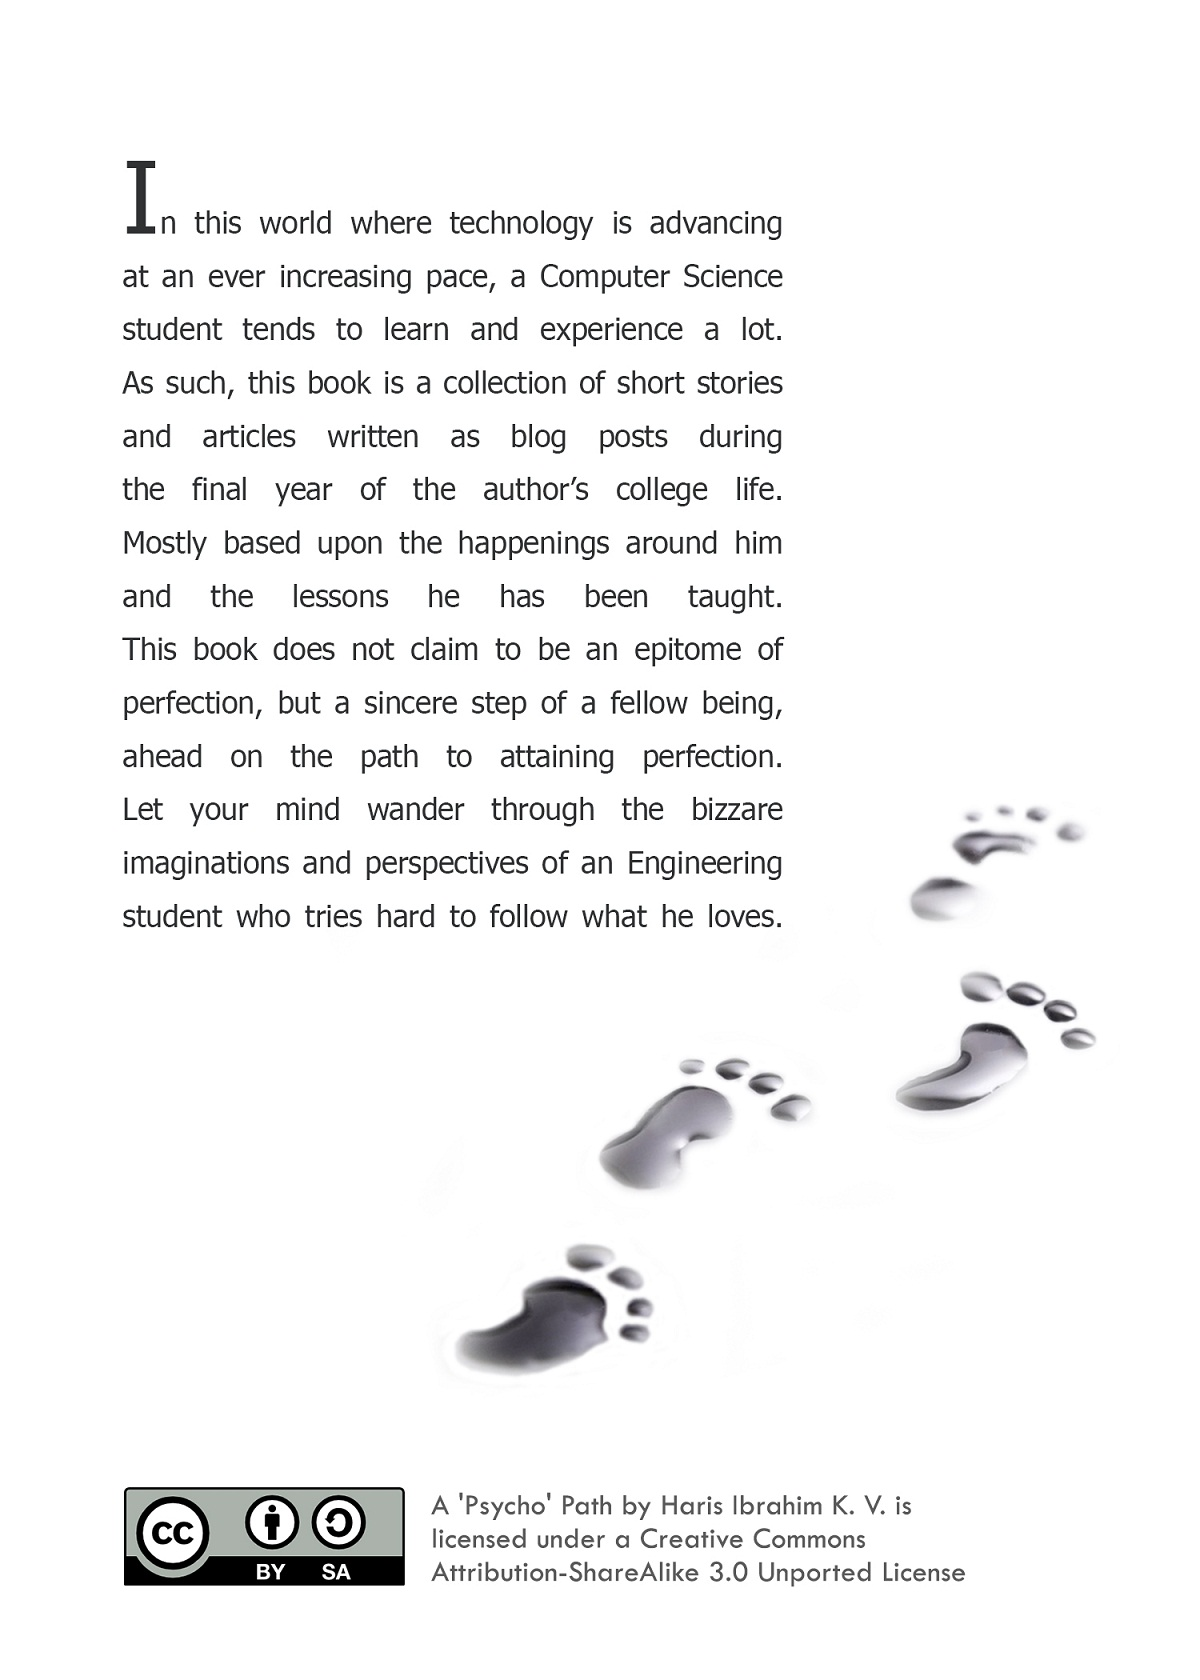
\includegraphics[width=\textwidth]{rear.jpg}
\end{textblock*}


\end{document}

